% !TEX program = latexmk
% A4 计算书
% UTF8 编码
\documentclass[a4paper,UTF8]{book}
% 中文环境
\usepackage{ctex}
% 页边距
\usepackage{geometry}
    \geometry{top = 0.8 in}
    \geometry{bottom = 1 in}
    \geometry{left = 0.5 in}
    \geometry{right = 0.5 in}
% 页眉和页脚设置
\usepackage{fancyhdr}
    \pagestyle{fancy}
    \fancyhead{}
    \fancyhead[LO,RE]{{\arabic{chapter}}}
    \fancyhead[RO,LE]{\rightmark}
% 中文章节号
% Chinese title
\usepackage{titlesec}
\titleformat{\chapter}{\centering\Huge\bfseries}{第\,\thechapter\,章}{1em}{}
% formulas
\usepackage{amsmath}
% table
\usepackage{booktabs}
% pictures
\usepackage{graphicx}
%  文章开始
% document
\begin{document}

% 封面
% ---------------------------------------------------------------------------
% cover
% 空页面设置
\thispagestyle{empty}
% 居中
\begin{center}
    % 和页眉距离
    \vspace*{3 cm}
    % 计算书标题:项目名称 + 换行计算书名称
    \heiti{\Huge{钢结构设计计算实例 \\ 钢结构屋盖系统}}\\
    \vspace*{3 cm}
    % 标题和图片距离
    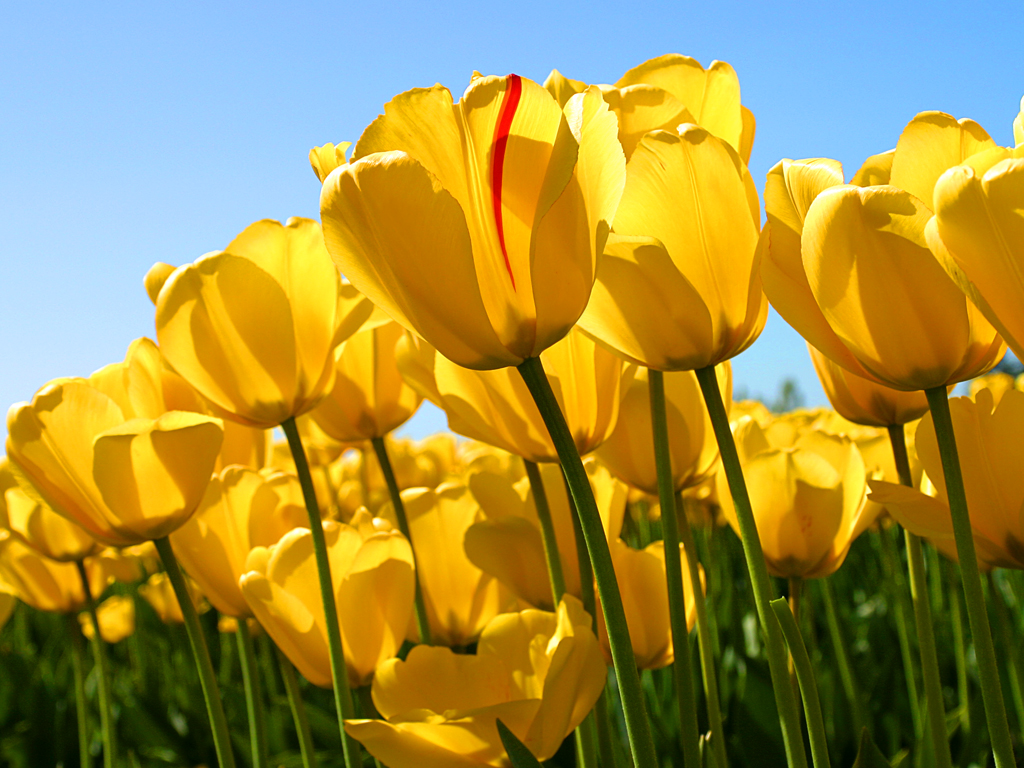
\includegraphics[width = 3 in]{cover.jpg}\\
    % 图片和日期距离
    \vspace*{5 cm}
    % 日期
    \Large {2019 年 11 月 15 日}\\
    % 日期和作者距离
    \vspace*{0.5cm}
    % 作者
    Will Clark\\
\end{center}
% \vspace*{4cm}
% 以下无内容
\clearpage

% 封二
% ---------------------------------------------------------------------------
% cover 2
% 新起一页
\newpage
% 空页面设置
\thispagestyle{empty}
% 顶格写
\noindent
书名: 《模板项目计算书》\\
作者: Will Clark\\
出版: 某出版社\\
版次: 2019 年 4 月 第 1 版\\
书号: ISBN 2-124-xxxx
% 以下无内容
\clearpage

% 目录
% ---------------------------------------------------------------------------
% 起始页码 1
% 目录页码
\setcounter{page}{1}
% 页码字体:罗马字体
\pagenumbering{Roman}
% 目录
\tableofcontents
% \thispagestyle{empty}
% 以下无内容
\clearpage

% 正文
% ---------------------------------------------------------------------------
% 起始页码 1
% 正文页码
\setcounter{page}{1}
% 页码字体:阿拉伯数字
\pagenumbering{arabic}

\chapter{跨度 $L = 6m$ 的槽钢简支试檩条}

\section{设计资料}
工程概况如下:
\paragraph{
    某工程厂房(封闭式)双坡屋面
}
$a = #a$,
$b = #b$。

\section{计算过程}
计算过程如下:
\begin{align*}
    c &= a + b \\
      &= #a + #b \\
      &= #c
\end{align*}

\section{计算结果}
求出结果:$c = #c$。

\end{document}
